\documentclass[xcolor={pst,x11names},compress]{beamer}

\usepackage{epsfig}
\usepackage{epstopdf}
\usepackage{tabularx}
\usepackage{graphicx}
\usepackage[round]{natbib}
\usepackage{transparent}
\usepackage{tikz}
\definecolor{emoryblue}{RGB}{0,40,120}
\definecolor{emorygray}{RGB}{91,92,94}
\definecolor{emorygold}{RGB}{210,176,0}
\usefonttheme{serif}
\usepackage{palatino}

\setbeamerfont{frametitle}{shape=\scshape}

\setbeamercolor*{lower separation line head}{bg=DeepSkyBlue4}
\setbeamercolor*{normal text}{fg=black,bg=white}
\setbeamercolor*{alerted text}{fg=red}
\setbeamercolor*{example text}{fg=black}
\setbeamercolor*{structure}{fg=black}

\setbeamercolor*{palette tertiary}{fg=black,bg=white!10}
\setbeamercolor*{palette quaternary}{fg=black,bg=black!10}

\renewcommand{\(}{\begin{columns}}
\renewcommand{\)}{\end{columns}}
\newcommand{\<}[1]{\begin{column}{#1}}
\renewcommand{\>}{\end{column}}
\newcommand{\semitransp}[2][35]{\color{fg!#1}#2}
\newcommand\T{\rule{0pt}{2.6ex}}
\newcommand\B{\rule[-1.2ex]{0pt}{0pt}}

\newcommand\Fontvi{\fontsize{6.8}{7.5}\selectfont}

\defbeamertemplate{footline}{centered frame number}
{%
  \hspace*{12cm}%
  \usebeamercolor[fg]{page number in head/foot}%
  \usebeamerfont{page number in head/foot}%
  \insertframenumber\,/\,\inserttotalframenumber%
 % \hspace*{\fill}
 \vskip2pt%
}
\setbeamertemplate{footline}[centered frame number]
\setbeamertemplate{footline}[frame number]
\setbeamertemplate{navigation symbols}{}
%%%%%%%%%%%%%%%%%%%%%%%%%%%%%%%%%%%%%%%%%%%%%%%
\setlength\labelsep   {\dimexpr\labelsep + 0.5em\relax}
\begin{document}
\addtocounter{framenumber}{-1}
\author[Adam Glynn]{ \textsc{Adam Glynn}} 
\date{\textsc{\today}}
\titlegraphic{
\includegraphics[width=1cm]{logo_emory_h.eps}}
%\date{}
\title{\large \color{emoryblue}
\textsc{QTM 220\\\vspace{0.3cm} 
Introduction to Formal Causal Inference with Multiple Linear Regression}
}
\titlegraphic{%
\begin{center}

\includegraphics[width=3cm]{logo_emory_h.eps}
\end{center}}

\setbeamertemplate{title page}
  {\begin{center}
      {\usebeamerfont{title}\usebeamercolor[fg]{title}\inserttitle}\\\vspace{2.5cm}
      {\usebeamerfont{author}\usebeamercolor[fg]{author}\insertauthor}\\
      \insertdate\\
      \inserttitlegraphic
    \end{center}
    }
%
\begin{frame}[plain]
\maketitle
\end{frame}
%

\begin{frame}{Reading}

These notes correspond to the material from Ch. 2.2-2.3 of Hernan and Robins' \emph{What If?}, and Ch. 3.7e, 4.7, 7.6 of Wooldridge's \emph{Introductory Econometrics}. 

\end{frame}

\begin{frame}{Agenda}

\begin{itemize}
\item Multiple linear regression with randomized experiments
\item Conditionally randomized experiments and standardization 
\item MLR.4 and SLR.4 with conditionally randomized experiments and constant effects
\item General estimation of ATE with regression and nonconstant effects
\end{itemize}

\end{frame}

%\frame{
%\frametitle{Multiple Regression with a randomized experiment}
%
%\begin{itemize}
%\item We showed last week that a simple linear regression (SLR) will produce an unbiased estimate of the average treatment effect. 
%\item Often people include additional covariates in a multiple linear regression (MLR) with a randomized experiment to improve efficiency.
%\item Sometimes people include covariates and interaction terms
%\item The following slides discuss this logic of this approach.  
%\item With a binary outcome, multiple logistic regression is often used to include covariates and increase efficiency, but 
%\end{itemize}
%
%}


\frame{

\center
\LARGE 
Multiple Linear Regression with a Randomized Experiment

}

\frame{
\frametitle{Notation and Reading}

For consistency, I'm using the notation from Wooldridge 3.7e and 7.6 in this section of the notes. There is no required reading corresponding to this material, but those interested should consult Ch. 4 of Gerber and Green \emph{Field Experiments}. 


}



\frame{
\frametitle{Multiple Linear Regression with a randomized experiment}

\begin{itemize}
\item We showed last week that the slope from a simple linear regression (SLR) of the outcome on the treatment variable will produce an unbiased estimate of the average treatment effect (ATE) with randomized treatment assignment.  \pause
\item With randomized treatment assignment, the slope for the treatment variable in a multiple linear regression (MLR) still estimates the ATE.   \pause
\item Because of this, we oftens use MLR to include covariates when analyzing a randomized experiment to improve efficiency.
\end{itemize}

}





\frame{
\frametitle{Recall: Randomization Implies Independence}

Using Wooldridge notation, suppose six subjects were randomly assigned to $w=0$ and $w=1$ (also imagine these six subjects actually represent 600 subjects), and we measure a ``pre-treatment'' covariate $x$.  

\begin{center}
\begin{tabular}{cccc|ccc}
$i$ & $x_i$ &$w_i$ & $y_i$ & $y_i(1)$ & $y_i(0)$ & $y_i(1)-y_i(0)$ \\
\hline
1 & 0  & 1 & 70 & 70 & ? & ? \\
2 & 1 & 1 & 80 & 80 & ? & ? \\
3 &  1& 0 & 60 & ? & 60 & ? \\
4 & 0  & 0 & 70 & ? & 70 & ? \\
5 &  0 & 0 & 70 & ? & 70 & ? \\
6 & 1 & 0 & 80 & ? & 80 & ? \\
\end{tabular}
\end{center}

Randomization implies that $x$ is independent of $w$, which implies that $E[x|w=1] = E[x|w=0]$.

}


\frame{
\frametitle{Why independence in large samples?}


\begin{center}
\begin{tabular}{cccc|ccc}
$i$ & $x_i$ &$w_i$ & $y_i$ & $y_i(1)$ & $y_i(0)$ & $y_i(1)-y_i(0)$ \\
\hline
1 & 0  & 1 & 70 & 70 & ? & ? \\
2 & 1 & 1 & 80 & 80 & ? & ? \\
3 &  1& 0 & 60 & ? & 60 & ? \\
4 & 0  & 0 & 70 & ? & 70 & ? \\
5 &  0 & 0 & 70 & ? & 70 & ? \\
6 & 1 & 0 & 80 & ? & 80 & ? \\
\end{tabular}
\end{center}

\begin{itemize}
\item The $w=1$ rows are a random sample of the rows, therefore $E[x|w=1] = E[x]$. 
\item The $w=0$ rows are a random sample of the rows, therefore $E[x|w=0] = E[x]$.
\item Therefore $E[x|w=1] = E[x|w=0]$.
\end{itemize}

}


%\begin{frame}[fragile]
%\frametitle{Recall: What if $w$ and $x$ are uncorrelated?}
%
%\begin{verbatim}
%> x <- rnorm(n)
%> w <- rnorm(n) # no x
%> cor(x,w)
%[1] 0.01075281
%> y <- w + x + rnorm(n)
%> lm(y ~ w)
%Coefficients:
%(Intercept)            w  
%    0.01027      1.00940  
%
%> lm(y ~ w + x)
%
%Coefficients:
%(Intercept)            w            x  
%    0.00417      0.99901      0.98509  
%    \end{verbatim}
%
%\end{frame}

\frame{
\frametitle{The Social Pressure Experiment}

\begin{center}
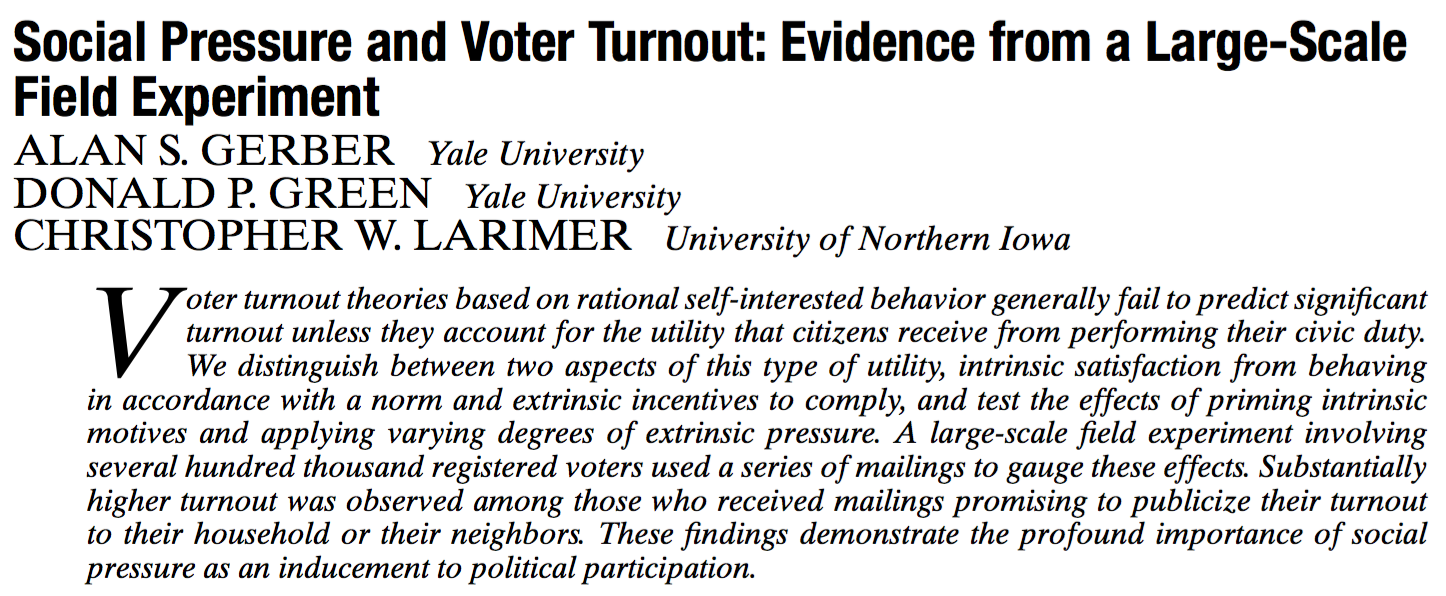
\includegraphics[width=4in]{figures/abstractGGL}
\end{center}

}

%\frame{
%\frametitle{The Civic Duty Treatment}
%
%\begin{center}
%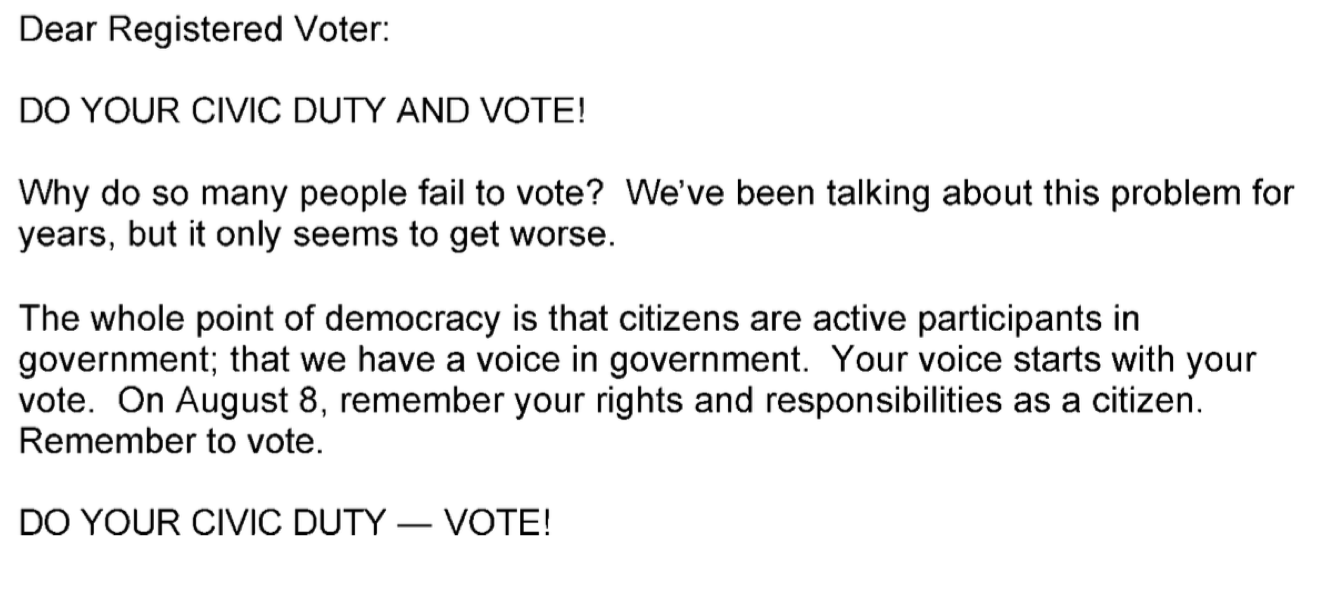
\includegraphics[width=4in]{figures/CivicDutyGGL}
%\end{center}
%
%}
%
%\frame{
%\frametitle{The Hawthorne Treatment}
%
%\begin{center}
%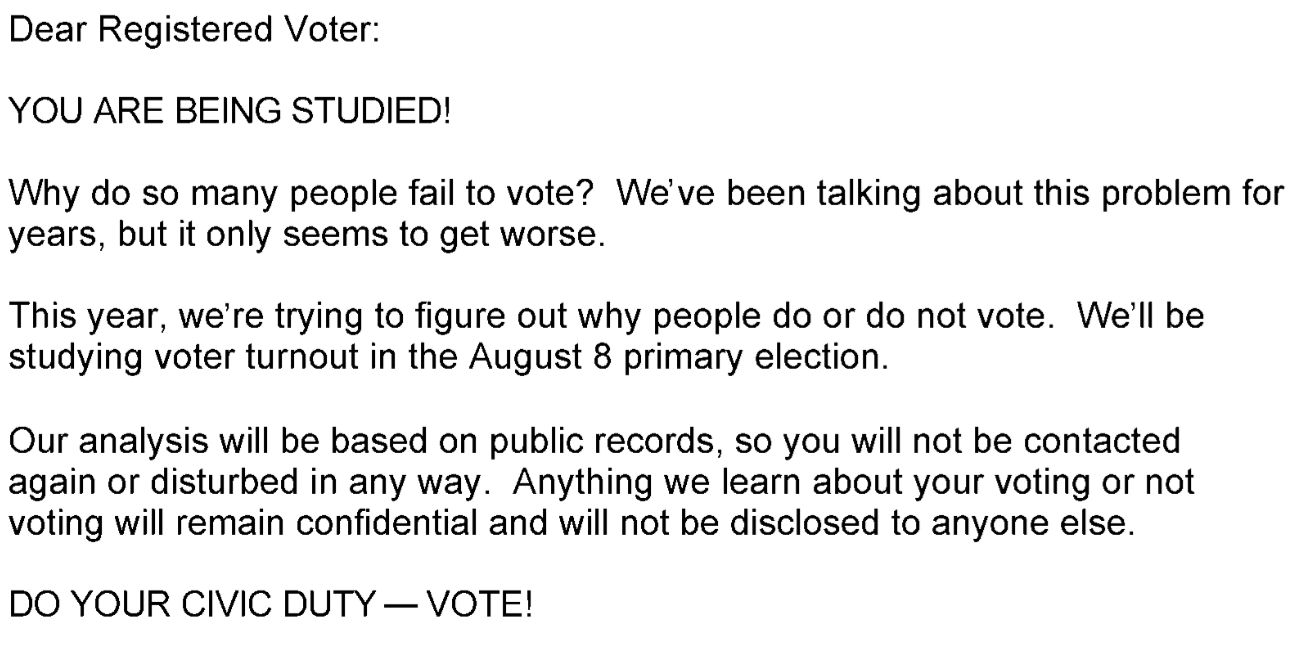
\includegraphics[width=4in]{figures/HawthorneGGL}
%\end{center}
%
%}
%
%\frame{
%\frametitle{The Self Treatment}
%
%\begin{center}
%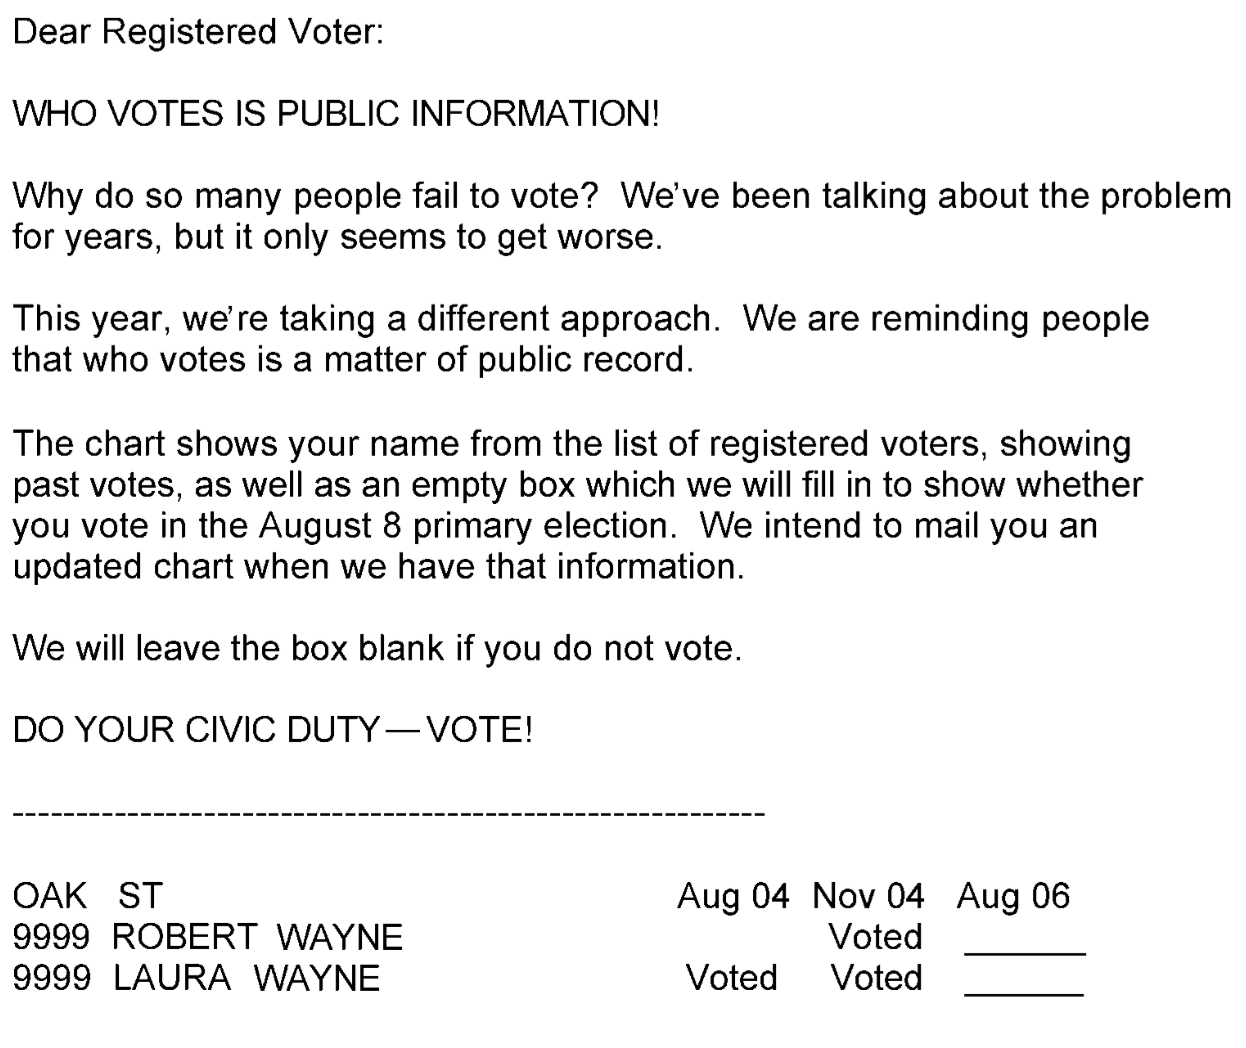
\includegraphics[width=3.5in]{figures/SelfGGL}
%\end{center}
%
%}

\frame{
\frametitle{The Neighbors Treatment}

\begin{center}
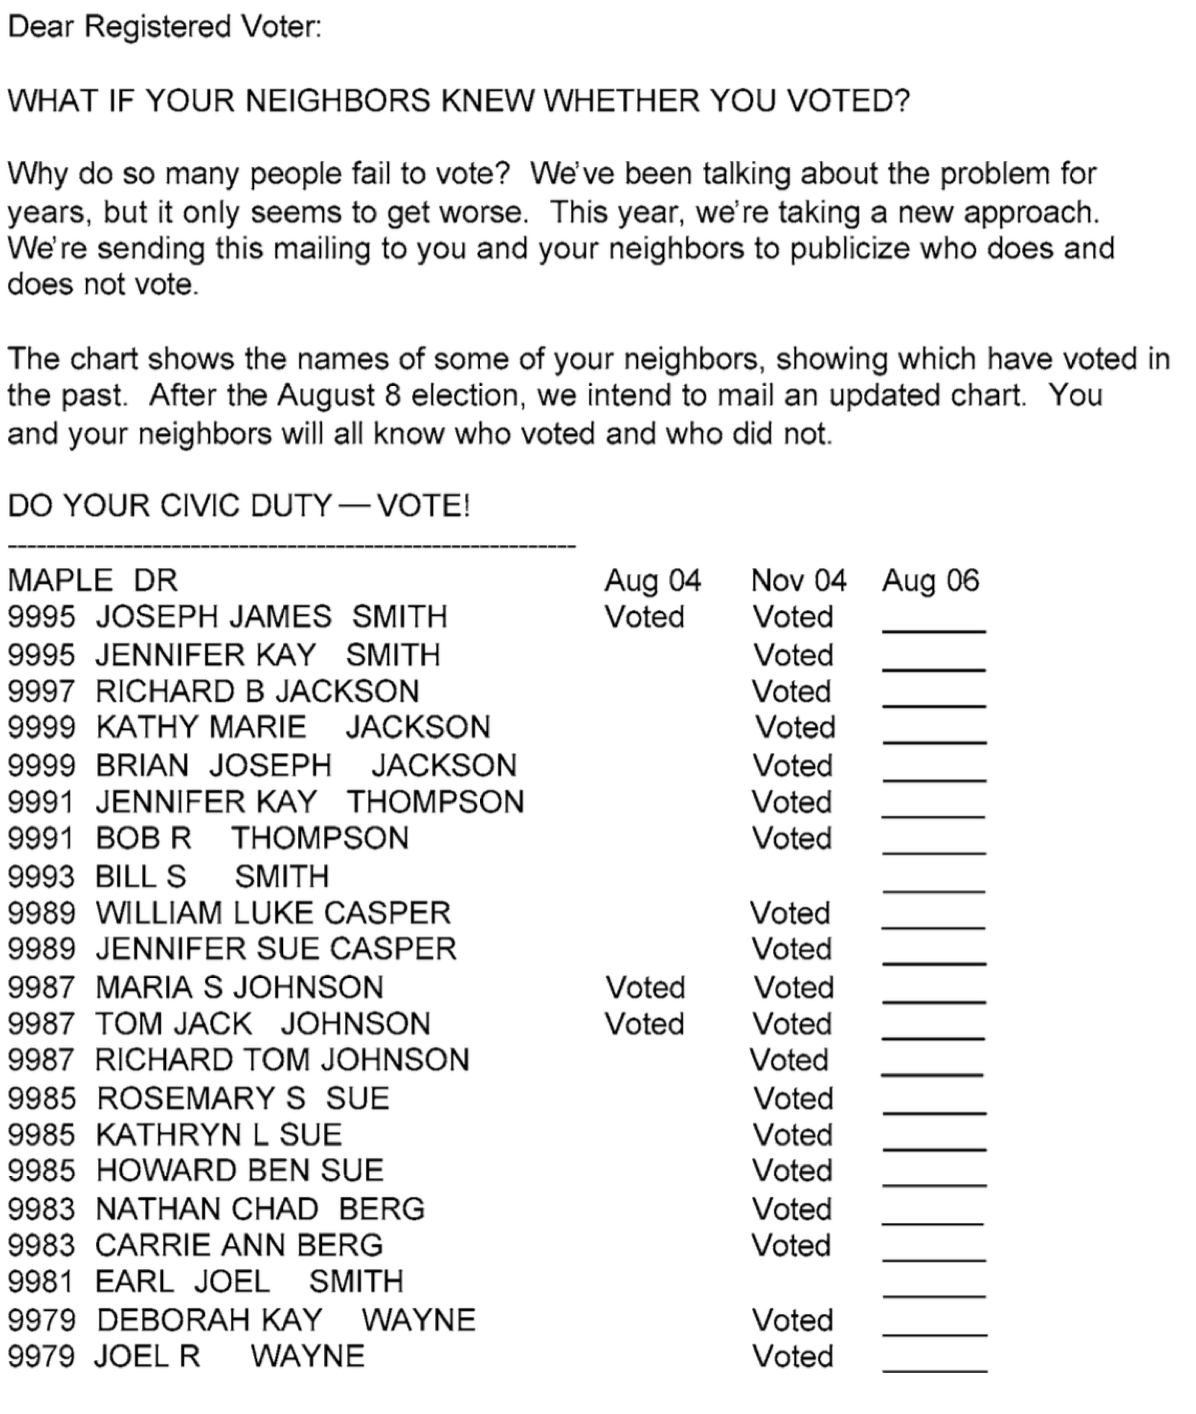
\includegraphics[width=3.5in]{figures/NeighborsGGL}
\end{center}

}

\frame{
\frametitle{Independence between Pre-treatment Variables and treatments in the GGL Experiment}

\begin{center}
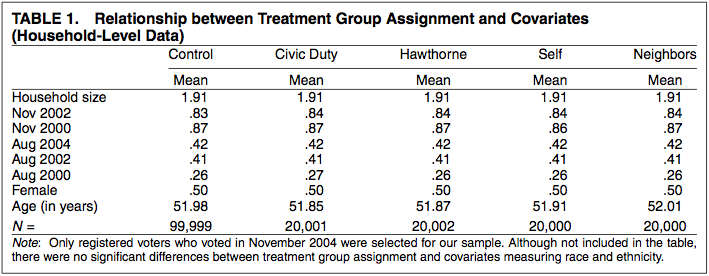
\includegraphics[width=4in]{lec15experiments/GGL}
\end{center}

}



\frame{
\frametitle{Including Covariates in the GGL Experiment}

\begin{center}
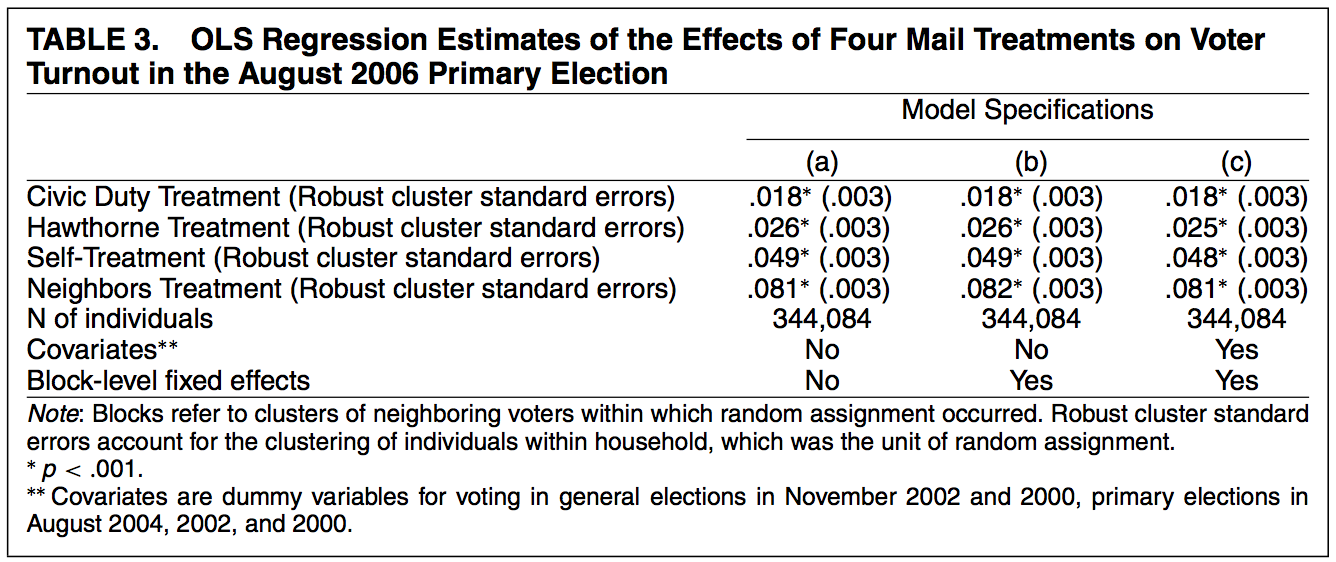
\includegraphics[width=4in]{lec15experiments/GGL2}
\end{center}

}

\frame{
\frametitle{Warning: Independence only for pre-treatment x}

\begin{itemize}
\item If $x$ is affected by $w$, then the previous results will not hold.
%\item Even though the $w=1$ rows are a random sample of the rows, $E[x|w=1] \ne E[x]$. 
%\item Even though the $w=0$ rows are a random sample of the rows, $E[x|w=0] \ne E[x]$.
%\item Therefore $E[x|w=1] \ne E[x|w=0]$.
\item Suppose $y=1$ indicates a heart attack, $w=1$ is a blood pressure medicine, and $x$ is post-treatment blood pressure. $x$ will be affected by $w$ and will therefore not be independent of $w$
\end{itemize}

}


\frame{
\frametitle{SLR vs MLR with Randomized $w$}

\begin{itemize}
\item In very large samples, MLR will produce approximately the same answer as SLR for the ATE (e.g., social pressure). \pause
\item In medium/large samples, (roughly $> 30$ d.f.), multiple linear regression will have small bias but will generally be more efficient than simple linear regression. \pause
\item In small samples, the bias in multiple linear regression will be too much.  \pause
\item The $x$ variables can include polynomials and interaction terms, but if $w$ is interacted with any $x$, then $\beta_w$ will no longer estimate ATE. \pause
\item This result holds for linear models used with limited dependent variables (LDV) such as the linear probability model when used with binary $y$, but robust SEs must be used. 
\end{itemize}

}




\frame{
\frametitle{Interactions and LDVs}

\begin{itemize}
\item There can be small sample advantages to interacting $w$ with the $x$ variables but the APE should be used to estimate the ATE (see Ch. 6-2d on Wooldridge pp. 194-195). \pause
\item There can be small sample advantages to using LDV models such as logit, but the APE should be used to estimate the ATE (e.g., see formula 17.17 on Wooldridge pg. 567 for the logit model).
\end{itemize}

}



\frame{

\center
\LARGE

Conditionally Randomized Experiments 

}

\frame{
\frametitle{Notation and Reading}

For consistency, I'm using the notation from Wooldridge 3.7e and 7.6 in this section of the notes, but this material corresponds to the reading from Ch. 2.2-2.3 of Hernan and Robins \emph{What If}. 


}


\frame{
\frametitle{Conditionally Randomized Experiment }


Suppose for one group/block/stratum ($\textcolor{green}{x=1}$) a coin was flipped to assign treatment to half of the units, and for another group/block stratum ($\textcolor{blue}{x=0}$), one out of four units was assigned to treatment. This is called a blocked, stratified, or conditionally randomized experiment. Essentially, we now have two experiments. 

\begin{center}
\begin{tabular}{cccc|ccc}
$i$ & $x_i$ & $w_i$ & $y_i$ & $y_i(1)$ & $y_i(0)$ & $y_i(1)-y_i(0)$ \\
\hline
1 & \textcolor{blue}{0} &1 & 70 & \textcolor{blue}{70} & ? & ? \\
2 & \textcolor{green}{1} &1 & 80 & \textcolor{green}{80} & ? & ? \\
3 & \textcolor{blue}{0} & 0 & 60 & ? & \textcolor{blue}{60} &?\\
4 & \textcolor{green}{1} &0& 70 & ? & \textcolor{green}{70} & ? \\
5 & \textcolor{blue}{0} & 0&70 & ? & \textcolor{blue}{70} & ? \\
6 & \textcolor{blue}{0}& 0 & 80 & ? & \textcolor{blue}{80} & ? \\
\end{tabular}
\end{center}

}

\frame{
\frametitle{Conditionally Randomized Experiment}

Within each of our two groups ($\textcolor{blue}{x=0}$ and $\textcolor{green}{x=1}$), all the properties discussed last week hold. Within $\textcolor{blue}{x=0}$,

\begin{center}

\begin{tabular}{cccc|ccc}
$i$ & $x_i$ & $w_i$ & $y_i$ & $y_i(1)$ & $y_i(0)$ & $y_i(1)-y_i(0)$ \\
\hline
1 & \textcolor{blue}{0} &1 & 70 & \textcolor{blue}{70} & \alert{70} & \alert{0} \\
2 & \textcolor{green}{1} &1 & 80 & \textcolor{green}{80} & \alert{70} & \alert{10} \\
3 & \textcolor{blue}{0} & 0 & 60 & \alert{60} & \textcolor{blue}{60} & \alert{0}\\
4 & \textcolor{green}{1} &0& 70 & \alert{80} & \textcolor{green}{70} & \alert{10} \\
5 & \textcolor{blue}{0} & 0&70 & \alert{70} & \textcolor{blue}{70} & \alert{0} \\
6 & \textcolor{blue}{0}& 0 & 80 & \alert{80} & \textcolor{blue}{80} & \alert{0} \\
\end{tabular}\\
\alert{remember red numbers not observed}
\end{center}


\visible<1-2>{What is the average $y_i(1)$ among the $x=0$ subjects?} 
\visible<2>{$$
\frac{\textcolor{blue}{70} +\alert{60} +\alert{70} + \alert{80}}{4}  = 70
$$}
\vspace{-2.4cm}

\visible<3-4>{What is the average $y_i(1)$ among the $x=0$, $w=1$ subjects?} 
\visible<4>{$$
\frac{\textcolor{blue}{70} }{1}  = 70
$$}
\vspace{-2.4cm}

\visible<5-6>{What is the average $y_i(0)$ among the $x=0$ subjects?} 
\visible<6>{$$
\frac{\textcolor{red}{70} +\textcolor{blue}{60} +\textcolor{blue}{70}+\textcolor{blue}{80}}{4}  = 70
$$}
\vspace{-2.4cm}

\visible<7-8>{What is the average $y_i(0)$ among the $x=0$, $w=0$ subjects?} 
\visible<8>{$$
\frac{\textcolor{blue}{60} +\textcolor{blue}{70}+\textcolor{blue}{80}}{3}  = 70
$$}

}

\frame{
\frametitle{Conditional ATE for $\textcolor{blue}{x=0}$}

Because we have a randomized experiment within the  $\textcolor{blue}{x=0}$ group and because of the linearity of expectations, the SLR slope (difference in means) among the $\textcolor{blue}{x=0}$ group provides an unbiased estimator of the conditional average treatment effect ($CATE_{x=0}$). 

\begin{align*}
&\frac{\textcolor{blue}{70} }{1}  - \frac{\textcolor{blue}{60} +\textcolor{blue}{70}+\textcolor{blue}{80}}{3} \\
&= \frac{\textcolor{blue}{70} +\alert{60} +\alert{70} + \alert{80}}{4} - \frac{\textcolor{red}{70} +\textcolor{blue}{60} +\textcolor{blue}{70}+\textcolor{blue}{80}}{4} \\
&= \frac{\alert{0} +\alert{0} +\alert{0} + \alert{0}}{4}
\end{align*}


}



\frame{
\frametitle{Conditionally Randomized Experiment}

Within the $\textcolor{green}{x=1}$ group, all the properties discussed last week hold.

\begin{center}
\begin{tabular}{cccc|ccc}
$i$ & $x_i$ & $w_i$ & $y_i$ & $y_i(1)$ & $y_i(0)$ & $y_i(1)-y_i(0)$ \\
\hline
1 & \textcolor{blue}{0} &1 & 70 & \textcolor{blue}{70} & \alert{70} & \alert{0} \\
2 & \textcolor{green}{1} &1 & 80 & \textcolor{green}{80} & \alert{70} & \alert{10} \\
3 & \textcolor{blue}{0} & 0 & 60 & \alert{60} & \textcolor{blue}{60} & \alert{0}\\
4 & \textcolor{green}{1} &0& 70 & \alert{80} & \textcolor{green}{70} & \alert{10} \\
5 & \textcolor{blue}{0} & 0&70 & \alert{70} & \textcolor{blue}{70} & \alert{0} \\
6 & \textcolor{blue}{0}& 0 & 80 & \alert{80} & \textcolor{blue}{80} & \alert{0} \\
\end{tabular}
\end{center}


\visible<1-2>{What is the average $y_i(1)$ among the $x=1$ subjects?} 
\visible<2>{$$
\frac{\textcolor{green}{80} +\alert{80} }{2}  = 80
$$}
\vspace{-2.4cm}

\visible<3-4>{What is the average $y_i(1)$ among the $x=1$, $w=1$ subjects?} 
\visible<4>{$$
\frac{\textcolor{green}{80}}{1}  = 80
$$}
\vspace{-2.4cm}

\visible<5-6>{What is the average $y_i(0)$ among the $x=1$ subjects?} 
\visible<6>{$$
\frac{\alert{70}  + \textcolor{green}{70}}{2}  = 70
$$}
\vspace{-2.4cm}

\visible<7-8>{What is the average $y_i(0)$ among the $x=1$, $w=0$ subjects?} 
\visible<8>{$$
\frac{\textcolor{green}{70}}{1}  = 70
$$}

}

\frame{
\frametitle{Conditional ATE for $\textcolor{green}{x=1}$}

Because we have a randomized experiment within the $\textcolor{green}{x=1}$ group and because of the linearity of expectations, the SLR slope (difference in means) among the $\textcolor{green}{x=1}$ group provides an unbiased estimator of the conditional average treatment effect ($CATE_{x=1}$). 

\begin{align*}
&\frac{\textcolor{green}{80} }{1}  - \frac{\textcolor{green}{70} }{1} \\
&=\frac{\textcolor{green}{80} +\alert{80} }{2} - \frac{\alert{70}  + \textcolor{green}{70}}{2} \\
&= \frac{\alert{10} +\alert{10}}{2}
\end{align*}


}




\frame{
\frametitle{Standardization}


If we average the $CATE_{x=0}$ and $CATE_{x=1}$ by the proportion in each group/block/stratum, then we get the ATE. In epidemiology, this is known as standardization.

\begin{center}
\begin{tabular}{cccc|ccc}
$i$ & $x_i$ & $w_i$ & $y_i$ & $y_i(1)$ & $y_i(0)$ & $y_i(1)-y_i(0)$ \\
\hline
1 & \textcolor{blue}{0} &1 & 70 & \textcolor{blue}{70} & ? & ? \\
2 & \textcolor{green}{1} &1 & 80 & \textcolor{green}{80} & ? & ? \\
3 & \textcolor{blue}{0} & 0 & 60 & ? & \textcolor{blue}{60} &?\\
4 & \textcolor{green}{1} &0& 70 & ? & \textcolor{green}{70} & ? \\
5 & \textcolor{blue}{0} & 0&70 & ? & \textcolor{blue}{70} & ? \\
6 & \textcolor{blue}{0}& 0 & 80 & ? & \textcolor{blue}{80} & ? \\
\end{tabular}
\end{center}



\begin{align*}
\textcolor{blue}{\frac{4}{6}} \cdot \left\{\frac{70}{1} -  \frac{60+70+80}{3}\right\} &+ \textcolor{green}{\frac{2}{6}} \cdot \left\{\frac{80}{1} -  \frac{70}{1}\right\} \\
&= \frac{20}{6}
\end{align*}
}


\frame{
\frametitle{Standardization}


If we average the $CATE_{x=0}$ and $CATE_{x=1}$ by the proportion in each group/block/stratum, then we get the ATE. In epidemiology, this is known as standardization.

\begin{center}
\begin{tabular}{cccc|ccc}
$i$ & $x_i$ & $w_i$ & $y_i$ & $y_i(1)$ & $y_i(0)$ & $y_i(1)-y_i(0)$ \\
\hline
1 & \textcolor{blue}{0} &1 & 70 & \textcolor{blue}{70} & \alert{70} & \alert{0} \\
2 & \textcolor{green}{1} &1 & 80 & \textcolor{green}{80} & \alert{70} & \alert{10} \\
3 & \textcolor{blue}{0} & 0 & 60 & \alert{60} & \textcolor{blue}{60} & \alert{0}\\
4 & \textcolor{green}{1} &0& 70 & \alert{80} & \textcolor{green}{70} & \alert{10} \\
5 & \textcolor{blue}{0} & 0&70 & \alert{70} & \textcolor{blue}{70} & \alert{0} \\
6 & \textcolor{blue}{0}& 0 & 80 & \alert{80} & \textcolor{blue}{80} & \alert{0} \\
\end{tabular}
\end{center}



\begin{align*}
\textcolor{blue}{\frac{4}{6}} \cdot \left\{\frac{70}{1} -  \frac{60+70+80}{3}\right\} &+ \textcolor{green}{\frac{2}{6}} \cdot \left\{\frac{80}{1} -  \frac{70}{1}\right\} \\
&= \frac{20}{6} = \frac{\alert{10}+\alert{10}}{6}
\end{align*}
}

\frame{
\frametitle{Omitted variable bias with SLR}


If we ignore the groups, and run an SLR on the entire data, we get omitted variable bias.

\begin{center}
\begin{tabular}{cccc|ccc}
$i$ & $X_i$ & $T_i$ & $Y_i$ & $Y_i(1)$ & $Y_i(0)$ & $Y_i(1)-Y_i(0)$ \\
\hline
1 & \textcolor{blue}{0} &1 & 70 & \textcolor{blue}{70} & \alert{70} & \alert{0} \\
2 & \textcolor{green}{1} &1 & 80 & \textcolor{green}{80} & \alert{70} & \alert{10} \\
3 & \textcolor{blue}{0} & 0 & 60 & \alert{60} & \textcolor{blue}{60} & \alert{0}\\
4 & \textcolor{green}{1} &0& 70 & \alert{80} & \textcolor{green}{70} & \alert{10} \\
5 & \textcolor{blue}{0} & 0&70 & \alert{70} & \textcolor{blue}{70} & \alert{0} \\
6 & \textcolor{blue}{0}& 0 & 80 & \alert{80} & \textcolor{blue}{80} & \alert{0} \\
\end{tabular}
\end{center}


\visible<1-2>{What is the average $Y_i(1) - Y_i(0)$?} 
\visible<2>{
\begin{align*}
\frac{\alert{0} + \alert{10} + \alert{0} +  \alert{10} +\alert{0} +\alert{0}}{6}  &= \frac{20}{6}\\
&\approx 3.3\\
 &\ne \frac{\textcolor{blue}{70} +\textcolor{green}{80} }{2} -  \frac{\textcolor{blue}{60} +\textcolor{green}{70} +  \textcolor{blue}{70} +\textcolor{blue}{80} }{4}
\end{align*}}

}

\frame{
\frametitle{Summary of Conditionally Randomized Experiments}

\begin{itemize}
\item A conditionally randomized experiment can be analyzed as multiple experiments and these results can be combined with standardization. 
\item If you ignore the groups in a conditionally randomized experiment, and the probability of treatment assignment is different in the groups, then you will induce omitted variable bias. 
\end{itemize}

}

\frame{
\frametitle{Up Next}

In the synchronous session this week, we will connect these results to material from Wooldridge 3.7e, 4.7, and 7.6. Some foreshadowing:

\begin{itemize}
\item Many non-experimental studies can be thought of as approximating a conditionally randomized experiment. 
\item Wooldridge presents techniques in 7.6 that are equivalent to standardization when $x$ is discrete.
\item In 3.7e and 4.7, Wooldridge presents models and methods for constant effects. With constant effects, a regression of $y$ on $w$ and $x$ will be preferred to standardization. Without constant effects, a regression of $y$ on $w$ and $x$ will produce a weighted average treatment effect.
\end{itemize}

}

\frame{

\center
\LARGE

Synchronous Material

}


%\frame{
%\frametitle{Causal Inference with Constant Effects}
%
%Using 3.7e Wooldridge notation, the observed outcome can be related to the baseline potential outcome and the treatment effect,
%\begin{align*}
%y_i &= (1-w_i)y_i(0) + w_i y_i(1)\\
%&= y_i(0) + [ y_i(1)-y_i(0)] w_i \\
%&= y_i(0) + te_i w_i
%\end{align*}
%
%With constant treatment effects and relabeling, we get the SLR model.\\
%\bigskip
% 
%Let $\beta_0= E[y_i(0)]$, $u_i = y_i(0) - E[y_i(0)]$, and $\beta_1 = \tau = te_i$ for all $i$.
%\begin{align*}
%y_i &= y_i(0) + te_i w_i \\ 
%&= E[y_i(0)] + \tau w_i + [y_i(0) - E[y_i(0)]] \\
%&= \beta_0  + \beta_1 w_i + u_i
%\end{align*}
%
%}

\frame{
\frametitle{Random Treatment Assignment and SLR.4 with Constant Treatment Effects}

\begin{align*}
y_i &= y_i(0) + te_i w_i \\ 
&= E[y_i(0)] + \tau w_i +  [y_i(0) - E[y_i(0)]] \\
&= \beta_0  + \beta_1 w_i + u_i
\end{align*}

Randomized $w$ implies that $w$ is independent of $[y(0), y(1)]$

This implies that SLR.4 holds,
\begin{align*}
 E[u|w] &= E[y_i(0) - E[y_i(0)]|w]\\
  &=  E[y_i(0)|w] - E[E[y_i(0)]|w] \\
 &= E[y_i(0)] - E[y_i(0)] \\
 &=0
\end{align*}
 
}

\frame{
\frametitle{with Covariates with Constant Effects}

As discussed in the ``MLR with Randomized Experiments'' video, randomized $w$ also implies that $w$ is independent of $[y(0), y(1)]$ conditional on $\bold{x}$ (as long as $\bold{x}$ is not affected by $w$). Hence, with constant treatment effects, $y = y(0) + \tau w$ and 
\begin{align*}
E[y|w,\bold{x}]&= E[y(0)|w,\bold{x}] + E[\tau w|w,\bold{x}] \\ 
&= E[y(0)|w,\bold{x}] + \tau w  
\end{align*}
Now if we assume that $E[y(0)|\bold{x}] = \alpha + \bold{x} \gamma$ and write $u = y(0) - \alpha + \bold{x} \gamma$, then MLR.4 holds,

\begin{align*}
 E[u|w,x] &= E[y(0) - (\alpha + \bold{x} \gamma) |w,\bold{x}]\\
  &=  E[y(0)|w,\bold{x}] - (\alpha + \bold{x} \gamma)  \\
 &=  E[y(0)|\bold{x}] - (\alpha + \bold{x} \gamma)  \\
 &=  \alpha + \bold{x} \gamma - (\alpha + \bold{x} \gamma) \\
 &=0
\end{align*}
 
}

\frame{
\frametitle{Conditional vs Unconditional with constant effects}


If $w$ is randomized unconditionally (aka marginally),
\begin{itemize}
\item this implies that $w$ is independent of $[y(0), y(1)]$ and that $w$ is independent of $[y(0), y(1)]$ conditional on $\bold{x}$ (when $\bold{x}$ is not affected by $w$). Hence, SLR.4 and MLR.4 hold.\\ (Note that MLR.4 will hold for lots of different $\bold{x}$.)
\end{itemize}

\bigskip
\bigskip

If $w$ is randomized conditionally on $\bold{x}$,
\begin{itemize}
\item then $w$ is independent of $[y(0), y(1)]$ conditional on $\bold{x}$, but $w$ is \alert{not} independent of $[y(0), y(1)]$ unconditionally (unless $P(w=1|\bold{x}) = P(w=1)$)
\item If $E[y(0)|\bold{x}]$ is linear, then MLR.4 holds, but SLR.4 does not hold, and SLR will lead to omitted variable bias.
\end{itemize}
 
}





\frame{
\frametitle{Approximating Conditional Randomization}

In non-experimental studies, conditioning on variables $\bold{x}$ that affect both the treatment $w$ and the outcome $y$ will often lead to a better approximation of a conditionally randomized experiment than a simple regression of $y$ on $w$ will approximate an unconditionally randomized experiment. \\


\bigskip
\bigskip

In example 3.7 on pg. 101, we have
\begin{itemize}
\item $\widehat{earn98} = 10.61 - 2.05 train$ with $se_{train} = 0.48$
\item $\widehat{earn98} = 4.67 + 2.41 train + .373 earn96 + .363 educ - .181 age  + 2.48 married$ with $se_{train} = 0.44$
\end{itemize}

We conclude that SLR.4 likely does not hold. Whether MLR.4 holds approximately is debatable.  

}

\frame{
\frametitle{with Nonconstant Effects}

If $w$ is conditionally randomized on $\bold{x}$ or we think that $w$ is approximately independent of $[y(0), y(1)]$ conditional on $\bold{x}$, then we can estimate the ATE as 
\begin{align*}
\frac{1}{n} \sum_{i=1}^n &\{ \hat y_i(1) - \hat y_i(0) \} \\
\end{align*} 
For $\hat y_i(1)$
\begin{enumerate}
\item Fit a regression of $y$ on $\bold{x}$ for just the $w=1$ observations.
\item Using this regression, predict $\hat y_i$ using $\bold{x}_i$ for all observations (i.e., with $w_i=1$ and $w_i=0$)  
\end{enumerate}

For $\hat y_i(0)$
\begin{enumerate}
\item Fit a regression of $y$ on $\bold{x}$ for just the $w=0$ observations.
\item Using this regression, predict $\hat y_i$ using $\bold{x}_i$ for all observations (i.e., with $w_i=1$ and $w_i=0$)  
\end{enumerate}
\bigskip
\bigskip
Note that we haven't specified the type of regression.


%$$
%\frac{1}{n} \sum_{i=1}^n \{ \hat E[y_i|w=1,\bold{x}_i] - \hat E[y_i|w=0,\bold{x}_i] \}
%$$
}

\frame{
\frametitle{}

On Wooldridge pg. 247, we see that with linear models, this approach will produce

\begin{align*}
\hat y_i(0) &= \hat \alpha_0 + \hat \gamma_{0,1} x_{i1} +  \hat \gamma_{0,2} x_{i2} +\dots + \hat \gamma_{0,k} x_{i1k} \\
\hat y_i(1) &= \hat \alpha_1 + \hat \gamma_{1,1} x_{i1} +  \hat \gamma_{1,2} x_{i2} +\dots + \hat \gamma_{1,k} x_{i1k}
\end{align*}
with

\begin{align*}
\frac{1}{n} \sum_{i=1}^n &\{ \hat y_i(1) - \hat y_i(0) \} \\
&= (\hat \alpha_1 - \hat \alpha_0) +  (\hat \gamma_{1,1}-\hat \gamma_{0,1}) \bar{x}_1 + \dots + (\hat \gamma_{1,k}-\hat \gamma_{0,k}) \bar{x}_k 
\end{align*} 

\bigskip
\bigskip

Note that if we center the $\bold{x}$ variables such that their means are zero and this formula is greatly simplified. 

}

\frame{

\begin{enumerate}
\item Draw a picture demonstrating this linear approach with a single $x$. 
\item Draw a picture demonstrating this approach with nonlinearities in $x$. 
\item Draw a picture demonstrating this approach with logistic regression. 
\end{enumerate}

}



\frame{
\frametitle{Standard Errors}

Notice that these approaches are equivalent to the average partial effect (APE) approaches we studied previously. For standard errors,
\begin{enumerate}
\item Use the package (like the one we showed you for logit)
\item Bootstrap
\end{enumerate}
 
}

\frame{
\frametitle{How to choose $\bold{x}$}

VanderWeele and Shpitser (2011), ``A new criterion for confounder selection,'' \emph{Biometrics} proved that a disjunctive cause criterion was sufficient for $w$ to be independent of $[y(0), y(1)]$ conditional on $\bold{x}$.

\bigskip
\bigskip

Disjunctive Cause Criterion:
\begin{enumerate}
\item Assume there is a correct set of pre-treatment variables in our data.
\item Then a set $\bold{x}$ that includes all variables that affect $w$, $y$, or both $w$ and $y$, will be sufficient for $w$ to be independent of $[y(0), y(1)]$ conditional on $\bold{x}$. 
\end{enumerate}

}




\end{document}




%%%%%%%%%%%%%%%%%%%%%%%%%%%%%%

